\documentclass[12pt]{article}


% -------------------- PAQUETES --------------------
\usepackage[utf8]{inputenc}
\usepackage[spanish]{babel}
\usepackage[margin=2.54cm]{geometry}
\usepackage{graphicx}
\usepackage{xcolor}
\usepackage{enumitem}
\usepackage{parskip}
\usepackage{hyperref}
\usepackage{ulem} 
\usepackage{subcaption}
\usepackage{url}


% -------------------- CARGA DE ARCHIVOS EXTERNOS --------------------
% ----------------- UTILIDADES PARA DAR UN MEJOR FORMATO DE DOCUMENTO -----------------  


\definecolor{azul}{rgb}{0.0039, 0.3098, 0.6196}


% Formato para el indice general ...........
\makeatletter
    \renewcommand{\@dotsep}{1.5}
    \renewcommand{\l@section}{\@dottedtocline{1}{1.5em}{2.3em}}
    \renewcommand{\l@subsection}{\@dottedtocline{2}{3.8em}{3.2em}}
    \renewcommand{\l@subsubsection}{\@dottedtocline{3}{7.0em}{4.1em}}
\makeatother

% --------- COMANDOS PERSONALIZADOS PARA LA PORTADA DE LAS TAREAS, TRABAJOS Y PROYECTOS ---------

\newcommand{\rutaLogo}[1]{\newcommand{\RutaLogo}{#1}}
\newcommand{\tema}[1]{\newcommand{\Tema}{#1}}
\newcommand{\etiquetaAutores}[1]{\newcommand{\EtiquetaAutores}{#1}}
\newcommand{\alumno}[1]{\newcommand{\Alumno}{#1}}
\newcommand{\materia}[1]{\newcommand{\Materia}{#1}}
\newcommand{\docente}[1]{\newcommand{\Docente}{#1}}
\newcommand{\ciclo}[1]{\newcommand{\Ciclo}{#1}}
\newcommand{\fecha}[1]{\newcommand{\Fecha}{#1}}
\newcommand{\periodo}[1]{\newcommand{\Periodo}{#1}}



% -------------------- DEFINICIÓN DE LA PORTADA --------------------
\rutaLogo{../../../../docs/img/logo-ista.png}
\tema{\\ \vspace{0.5cm} Proceso de tratamiento de los datos en un conjunto de datos de ventas de llantas \\ \vspace{1.2cm}}
\etiquetaAutores{Integrantes:}
\alumno{Nube Gutierrez\\Eduardo Mendieta\vspace{0.7cm}}
\materia{Introducción a Big Data \vspace{0.7cm}}
\docente{MSc. Ing. Carmen Tacuri Vintimilla \vspace{0.7cm}}
\ciclo{Primer Ciclo \vspace{0.7cm}}
\fecha{18 de agosto de 2024 \vspace{0.7cm}}
\periodo{Abril 2024 - Agosto 2024}

\begin{document}

    \begin{titlepage}

    \centering

    \includegraphics[width=0.11\textwidth]{\RutaLogo} 

    \vspace{0.3cm}
    \textcolor{azul}{\Large \textbf{Instituto Superior Universitario Tecnológico del Azuay \\}}
    \vspace{0.3cm}
    \textcolor{azul}{\Large \textbf{Tecnología Superior en Big Data}}
    
    % 1. ---------------- TEMA -------------------------
    
    {\Large\textbf{\Tema}}
    
    % 2. ---------------- AUTOR(ES) -------------------------
    \textcolor{azul}{\large \textbf{\EtiquetaAutores} \\}
    \vspace{0.3cm}
    {\large \Alumno}

    % 3. ---------------- MATERIA -------------------------
    \textcolor{azul}{\large \textbf{Materia:} \\}
    \vspace{0.3cm}
    {\large \Materia}


    % 3. ---------------- DOCENTE -------------------------
    \textcolor{azul}{\large \textbf{Docente:} \\}
    \vspace{0.3cm}
    {\large \Docente}


    % 3. ---------------- Ciclo -------------------------
    \textcolor{azul}{\large \textbf{Ciclo:} \\}
    \vspace{0.3cm}
    {\large \Ciclo}


    % 3. ---------------- FECHA -------------------------
    \textcolor{azul}{\large \textbf{Fecha:} \\}
    \vspace{0.3cm}
    {\large \Fecha}

    % 3. ---------------- PERIODO -------------------------
    \textcolor{azul}{\large \textbf{Periodo Académico:} \\}
    \vspace{0.3cm}
    {\large \Periodo}
 
\end{titlepage}


    \tableofcontents
    \newpage

    \section*{\centering Proceso de tratamiento de los datos en un conjunto de datos de ventas de llantas}

    % 1.Introducción: ...................................................
    \section{Introducción}
    La visualización de datos es una técnica esencial en el análisis de datos que permite transformar grandes volúmenes de información compleja en representaciones gráficas comprensibles y significativas. Al utilizar gráficos, diagramas y mapas, la visualización facilita la identificación de patrones, tendencias y anomalías que podrían ser difíciles de detectar en datos crudos. Este enfoque no solo mejora la comunicación de los hallazgos de los datos, sino que también potencia la toma de decisiones informadas y estratégicas en diversos ámbitos.

    En el mundo del análisis de datos, existen numerosas herramientas diseñadas para crear visualizaciones efectivas. Programas como Tableau, Power BI y R con sus paquetes específicos, como ggplot2, ofrecen capacidades avanzadas para generar desde gráficos básicos hasta complejas visualizaciones interactivas. Estas herramientas permiten a los analistas explorar y presentar datos de manera intuitiva, adaptando las representaciones visuales a las necesidades específicas del análisis y del público objetivo. Con la creciente disponibilidad de herramientas y técnicas, la visualización de datos se ha convertido en una habilidad clave para transformar datos en insights valiosos.

    % 2.Objetivos: ...................................................
    \section{Objetivo}
        Realizar el proceso completo de tratamiento de datos, que incluye la preparación, limpieza y visualización de un conjunto de datos proporcionado por el docente.

    \section{Encuesta}

    Link para la \texttt{\textbf{\href{https://docs.google.com/forms/d/e/1FAIpQLSfqX3hlz6KKEy3PdoWKuSmd8aaH2FvSwmvK5ErNoTeH5opCoQ/viewform?usp=sf_link}{encuesta}.}}

    % 3.Paso a Paso: ...................................................
    \newpage
    \section{Paso a paso}
    
        Para la realización del proceso de tratamiento de datos, hemos elegido un conjunto de datos sobre ventas de llantas proporcionado en un archivo Excel y la herramienta R para su análisis, preparación y visualización. R es un lenguaje de programación y un entorno de software especializado en el análisis estadístico y la visualización de datos. Su amplia gama de paquetes y funciones permite transformar datos mediante técnicas avanzadas de manipulación y modelado, facilitando la limpieza, integración y análisis. Además, R destaca en la visualización de datos, ofreciendo herramientas para crear gráficos y visualizaciones interactivas y personalizables que ayudan a interpretar y comunicar resultados de manera efectiva. 
        
        A continuación, se detallan cada uno de los pasos realizados para completar este proceso:

        \subsection{Adquisición y preparación}
            
            \begin{itemize}
                \item El set de datos es el siguiente:
                    \begin{figure}[h]
                        \centering 
                        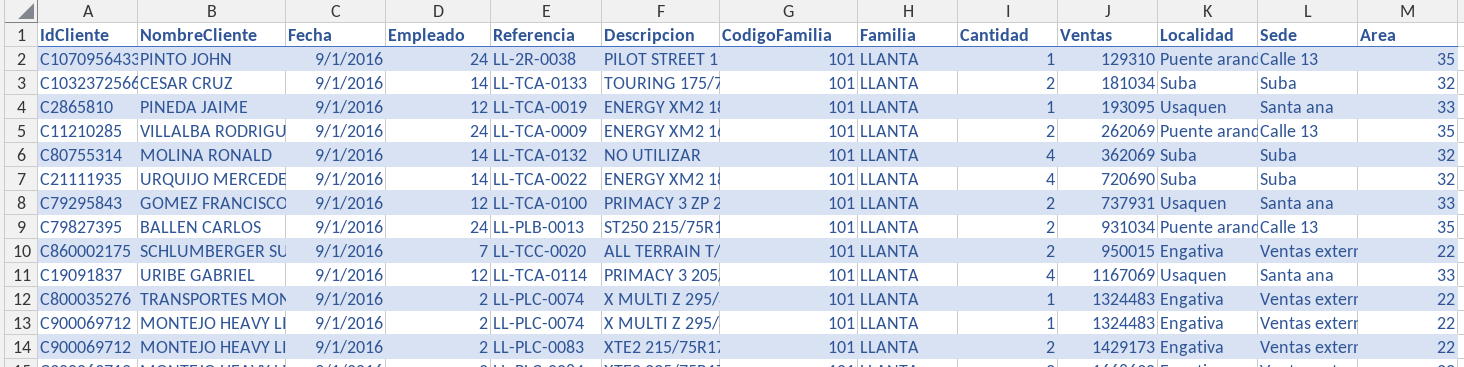
\includegraphics[width=1\textwidth]{img/limpieza-1.png}
                        \caption{Archivo Excel con los datos}
                \end{figure}

                \item Iniciamos creando un script en R en la misma carpeta en la que se encuentra el conjunto de datos. Una vez creado el script, Utilizamos la función \texttt{read\_excel()} de la biblioteca \texttt{readxl} para cargar los datos en el entorno de R.
                    \begin{figure}[h]
                        \centering 
                        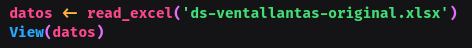
\includegraphics[width=0.7\textwidth]{img/limpieza-2.png}
                        \caption{Cargando los datos en R}
                    \end{figure}

                    \newpage
                    \begin{figure}[h]
                        \centering 
                        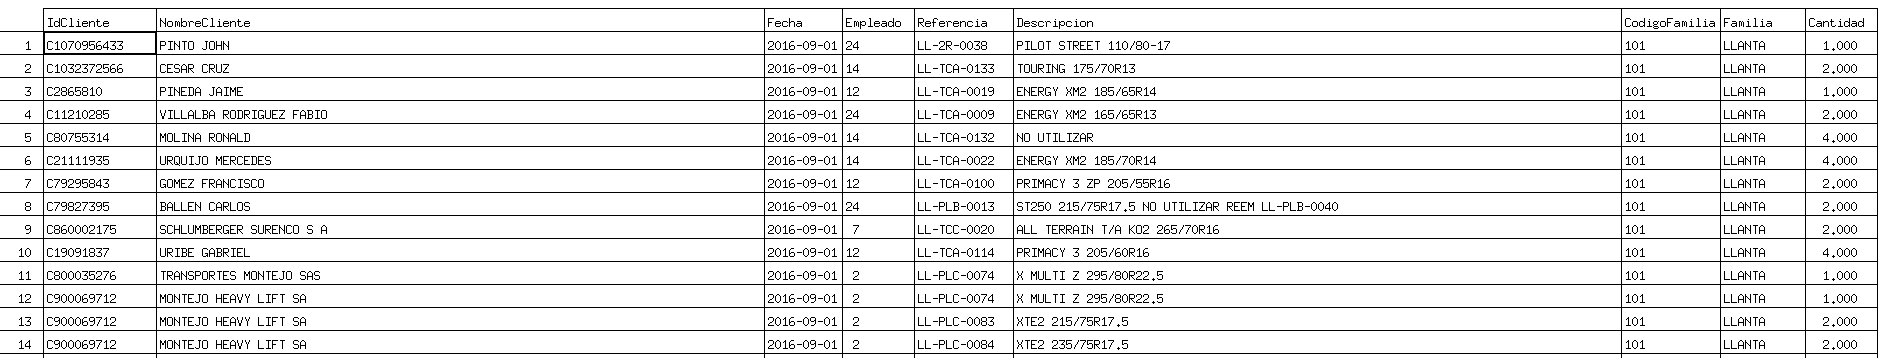
\includegraphics[width=1\textwidth]{img/limpieza-3.png}
                        \caption{Visualización de los datos en R}
                    \end{figure}

            \end{itemize}


        \subsection{Organización y limpieza}

            \begin{itemize}
                \item Usando la función \texttt{nrow()} podemos observar el conjunto de datos tiene \texttt{127266 filas}. Aplicamos un filtro para observar si existen filas que esten completamente en blanco y como resultado existen \texttt{11 filas}. Para eliminar dichas filas creamos una nueva variable que almacene los \texttt{datos limpios} y aplicando nuevamente el filtro extraemos unicamente la filas que contienen datos, quedando un total de \texttt{127255 filas}.
                    \begin{figure}[h]
                        \centering 
                        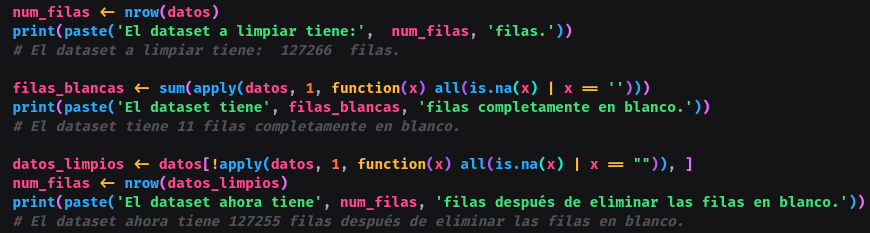
\includegraphics[width=1\textwidth]{img/limpieza-4.png}
                        \caption{Eliminando filas vacias}
                    \end{figure}

                \item Ordenamos las filas utilizando alguna columna con la función \texttt{arrange()} de la biblioteca \texttt{dplyr}, en este caso \texttt{Empleado}, con el objetivo de poder visualizar si existen filas duplicadas. Aplicamos un filtro para identificar y eliminar filas repetidas. En el conjunto de datos existen \texttt{24923 filas repetidas}, luego de este proceso, tendremos un total de \texttt{102332 filas}.
                    \begin{figure}[h]
                        \centering 
                        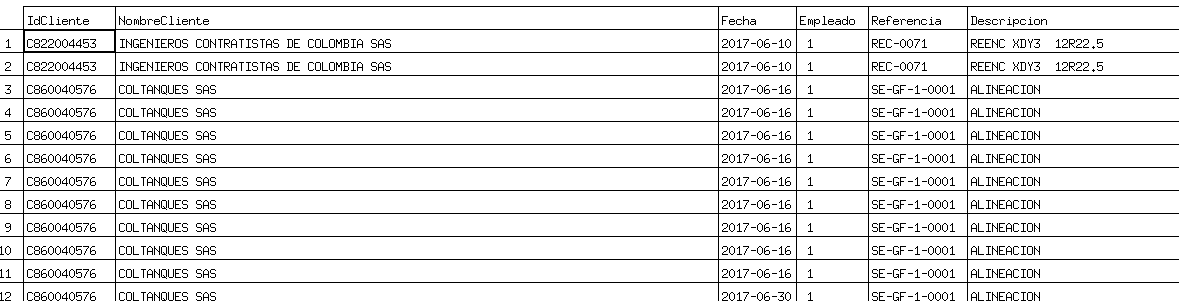
\includegraphics[width=1\textwidth]{img/limpieza-5.png}
                        \caption{Visualización de datos repetidos}
                    \end{figure}

                    \newpage
                    \begin{figure}[h]
                        \centering 
                        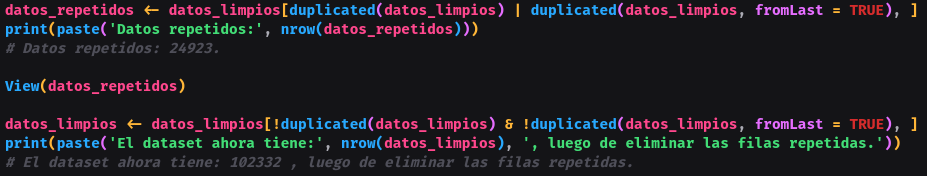
\includegraphics[width=1\textwidth]{img/limpieza-6.png}
                        \caption{Eliminando datos repetidos}
                    \end{figure}
                
                \item Buscamos el número de valores faltantes por columna utilizando la función \texttt{colSums()}, para aplicar cualquier operación de limpieza en el caso de encontrar datos faltantes. Podemos observar que el número de datos faltantes es \texttt{cero} en todas las columnas.
                    \begin{figure}[h]
                        \centering 
                        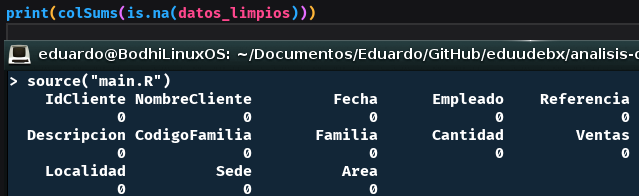
\includegraphics[width=0.8\textwidth]{img/limpieza-7.png}
                        \caption{Buscando datos faltantes por columna}
                    \end{figure}
                
                \item Validamos que las columnas \texttt{Empleado, CodigoFamilia, Ventas, Area} y \texttt{Cantidad}, tengan números enteros mayores a cero. Luego de la validación la unica que no cumplia con esta restricción es \texttt{Cantidad} puesto que tiene unicamente 2 celdas con valores decimales \texttt{'1.068, 1.006'} extos valores fueron redondeados al inmediato superior.
                    \begin{figure}[h]
                        \centering 
                        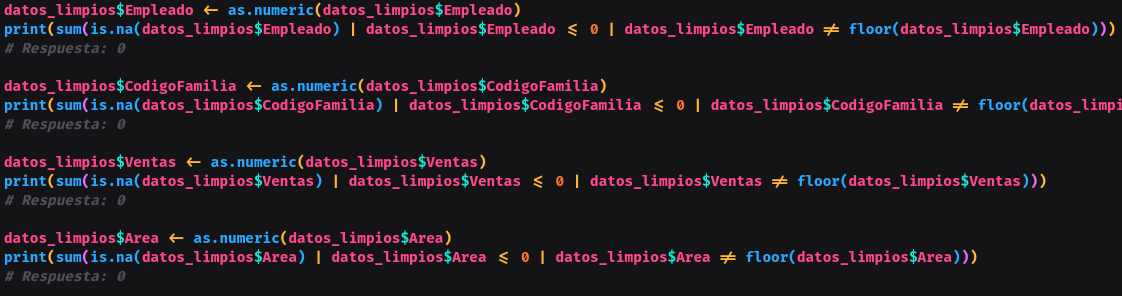
\includegraphics[width=1\textwidth]{img/limpieza-8.png}
                        \caption{Validando columnas con valores enteros}
                    \end{figure}

                    \newpage
                    \begin{figure}[h]
                        \centering 
                        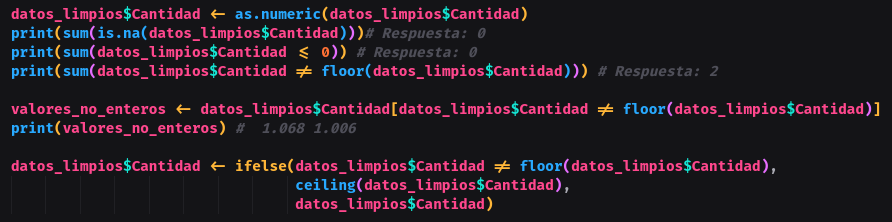
\includegraphics[width=1\textwidth]{img/limpieza-9.png}
                        \caption{Corrigiendo datos de la columna \texttt{Cantidad}}
                    \end{figure}
                
                \item En la columna \texttt{Fecha}, validamos que todos los campos tengan el formato \texttt{mes/dia/año}. Al realizar dicha validación, todos los campos cumplen con la condición. Procedemos a cambiar el formato de la fecha a \texttt{dia/mes/año}.
                    \begin{figure}[h]
                        \centering 
                        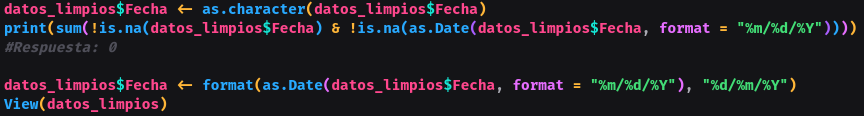
\includegraphics[width=1\textwidth]{img/limpieza-10.png}
                        \caption{Validando colunma de \texttt{Fecha}}
                    \end{figure}

                    \begin{figure}[h]
                        \centering 
                        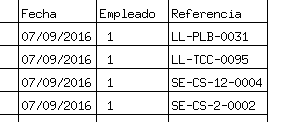
\includegraphics[width=0.6\textwidth]{img/limpieza-11.png}
                        \caption{Formato de fecha \texttt{dia/mes/año}}
                    \end{figure}
                
                
                \item En el caso de las columnas \texttt{NombreCliente, Descripcion, Familia, Localidad} y \texttt{ Sede} cambiamos su formato de texto a \texttt{capitalize} de tal modo que todas tengan el mismo formato. Esto utilizando la biblioteca \texttt{stringr}.
                    \newpage    
                    \begin{figure}[h]
                        \centering 
                        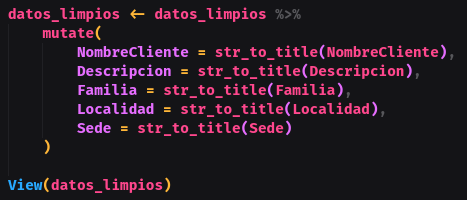
\includegraphics[width=0.5\textwidth]{img/limpieza-12.png}
                        \caption{Dando un unico formato a las columnas tipo \texttt{String}}
                    \end{figure}

                    \begin{figure}[h]
                        \centering 
                        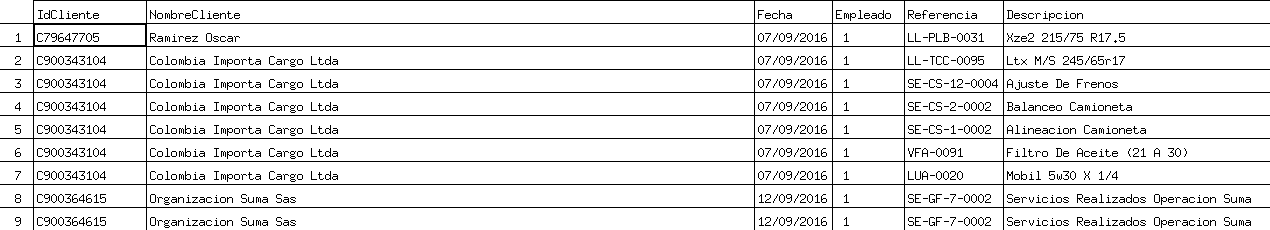
\includegraphics[width=1\textwidth]{img/limpieza-13.png}
                        \caption{Visualización del resultado final}
                    \end{figure}
                
                \item Una vez culminado el proceso de limpieza, de un total de \texttt{127266 registros} del set de datos original, el resultado es uno con \texttt{102332}. En total se han eliminado un total de \texttt{24934 registros}.
                    \begin{figure}[h]
                        \centering 
                        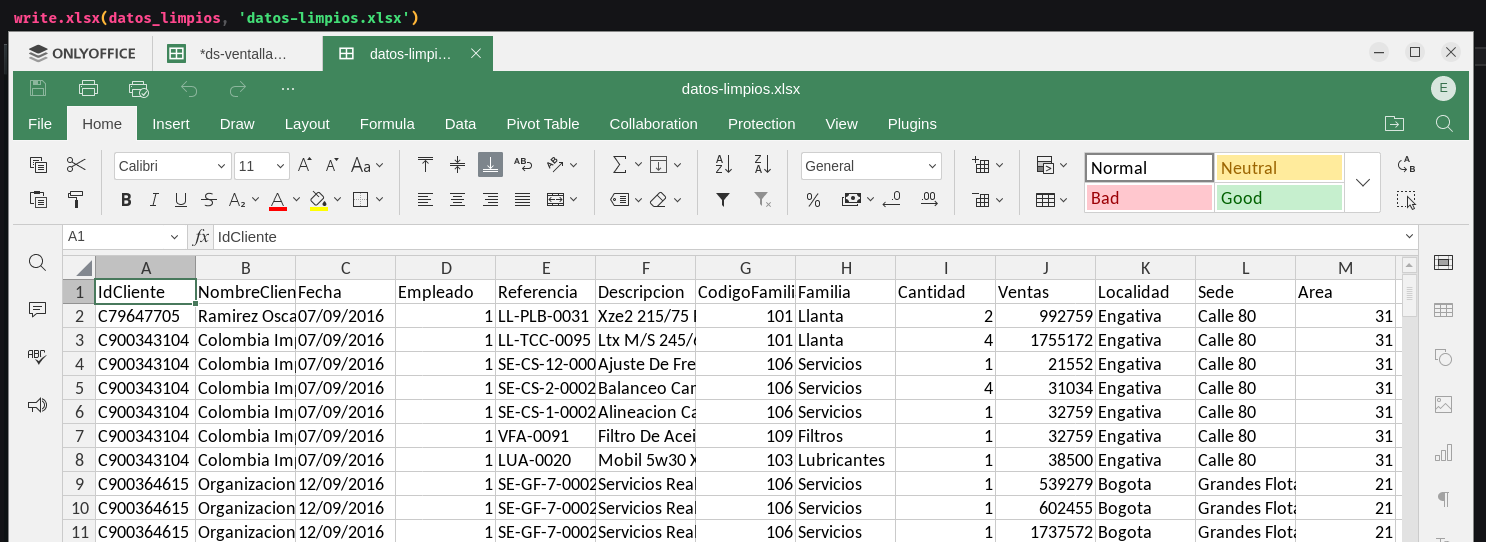
\includegraphics[width=1\textwidth]{img/limpieza-14.png}
                        \caption{Exportación de set de datos limpio}
                    \end{figure}
            
            \end{itemize}


        \newpage    
        \subsection{Transformación y visualización}
            Previo a la depuración de los datos, se generó un \texttt{Modelo Relacional} con el fin de darle estructura a la información y tener una idea de cómo deberíamos tratarla.
            \begin{figure}[h]
                \centering 
                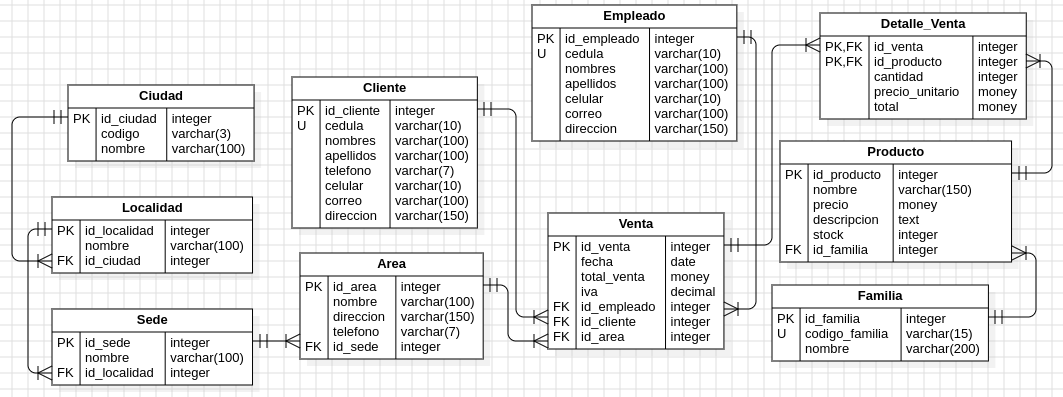
\includegraphics[width=1\textwidth]{img/transformacion-1.png}
                \caption{Modelo Físico - Relacional}
            \end{figure}

            \vspace{0.5cm}\textbf{Bibliotecas principales para la generación de gráficos en R} \vspace{0.5cm}
            
            \begin{enumerate}
                \item \textbf{ggplot2:}  Es una de las bibliotecas de visualización más populares en R. Basada en la gramática de gráficos, permite crear gráficos complejos a partir de componentes simples. Ofrece una amplia gama de gráficos, como histogramas, gráficos de dispersión, gráficos de barras, gráficos de líneas y gráficos de cajas.
                \item \textbf{base R:} La funcionalidad gráfica básica de R permite crear gráficos sin la necesidad de paquetes adicionales. Permite crear gráficos de dispersión, histogramas, gráficos de barras y gráficos de líneas con funciones como \texttt{plot()}, \texttt{hist()}, \textbf{barplot()} y \texttt{boxplot()}.
                \item \textbf{lattice:} Es una biblioteca que facilita la creación de gráficos de panel y gráficos condicionados. Ofrece gráficos multivariantes y permite la visualización de datos en paneles.
                \item \textbf{plotly:} Se integra con \texttt{ggplot2} para crear gráficos interactivos y visualizaciones dinámicas. Permite crear gráficos interactivos, mapas y otros tipos de visualizaciones que pueden ser manipuladas en tiempo real.
            \end{enumerate}

            \newpage\textbf{Dos Propuestas de gráficos en R} \vspace{0.5cm}

            \begin{itemize}
                \item La primera propuesta para la visualización de los datos en un \texttt{gráfico de barras} en el cual se analiza la cantidad de ventas realizadas por cada uno de los empleados en los distintos años. Para esto se creó una columna llamada \texttt{AnioVenta} y \texttt{NombreEmpleado} derivadas de \texttt{Fecha} y \texttt{Empleado} respectivamente.
                    \begin{figure}[h]
                        \centering 
                        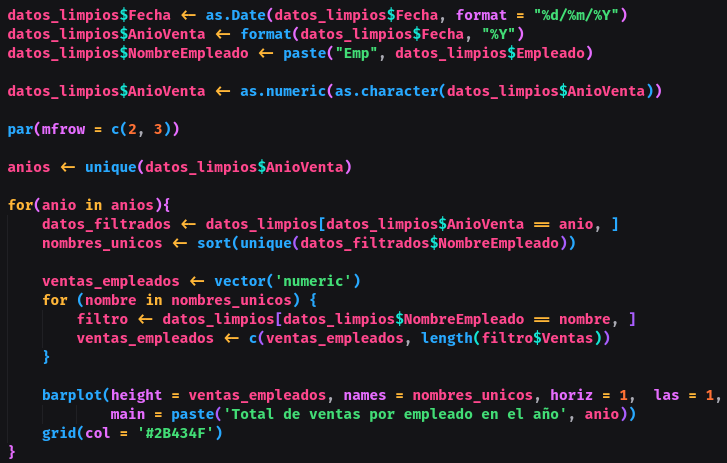
\includegraphics[width=0.7\textwidth]{img/visualizacion-1.png}
                        \caption{Filtro de datos para crear el grafico de barras}
                    \end{figure}

                    \begin{figure}[h]
                        \centering 
                        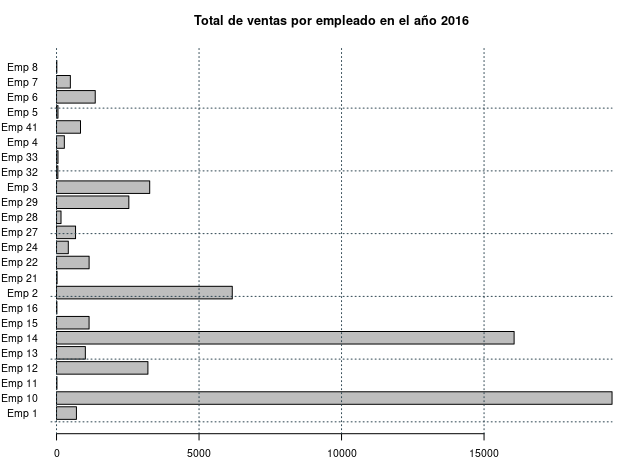
\includegraphics[width=0.6\textwidth]{img/grafico-barras-1.png}
                        \caption{Gráfico de barras 1}
                    \end{figure}

                    \newpage
                    \begin{figure}[h]
                        \centering 
                        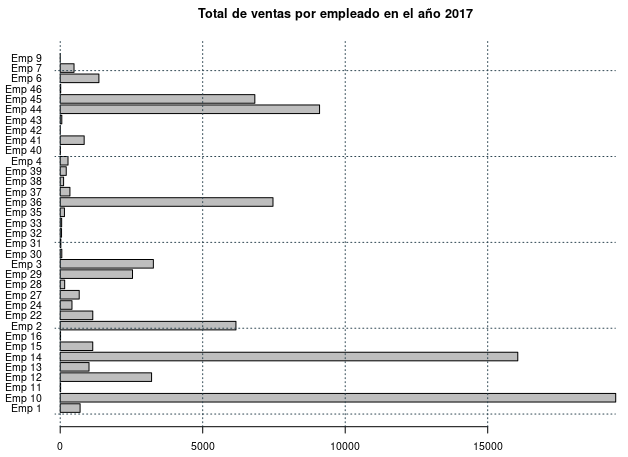
\includegraphics[width=0.6\textwidth]{img/grafico-barras-2.png}
                        \caption{Gráfico de barras 2}
                    \end{figure}

                    \begin{figure}[h]
                        \centering 
                        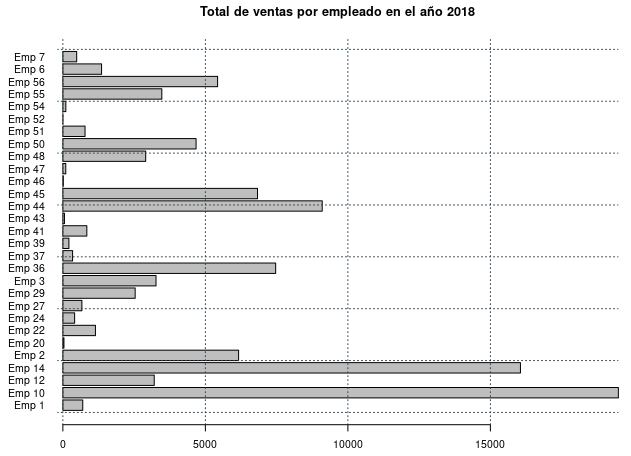
\includegraphics[width=0.6\textwidth]{img/grafico-barras-3.png}
                        \caption{Gráfico de barras 3}
                    \end{figure}

                    \newpage
                    \begin{figure}[h]
                        \centering 
                        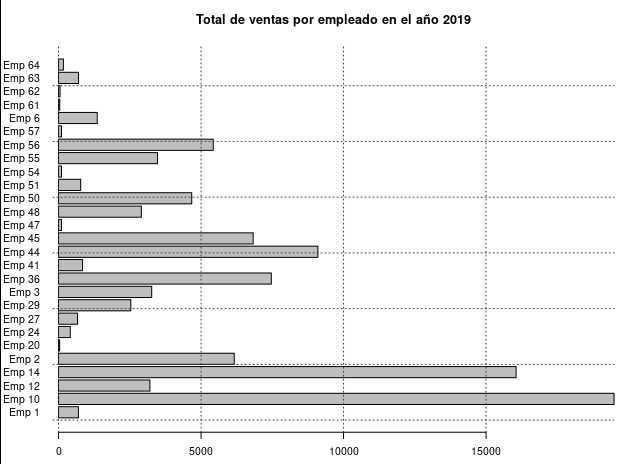
\includegraphics[width=0.6\textwidth]{img/grafico-barras-4.png}
                        \caption{Gráfico de barras 4}
                    \end{figure}

                    \begin{figure}[h]
                        \centering 
                        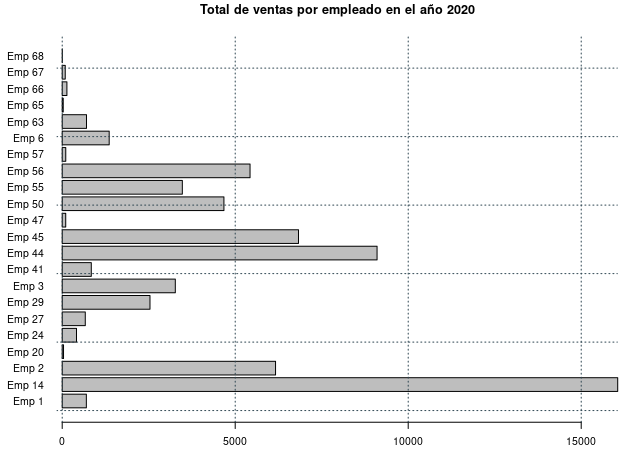
\includegraphics[width=0.6\textwidth]{img/grafico-barras-5.png}
                        \caption{Gráfico de barras 5}
                    \end{figure}

                \newpage
                \item Otra propuesta es un \texttt{Gráfico de pastel}, en este caso usamos la columna \texttt{Familia} para repreesentar el porcentaje de categorias vendidas en todos los años.
                    \begin{figure}[h]
                        \centering 
                        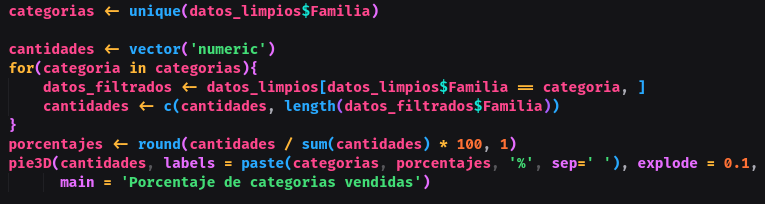
\includegraphics[width=0.8\textwidth]{img/visualizacion-2.png}
                        \caption{Filtro de datos para crear el grafico de barras}
                    \end{figure}

                    \begin{figure}[h]
                        \centering 
                        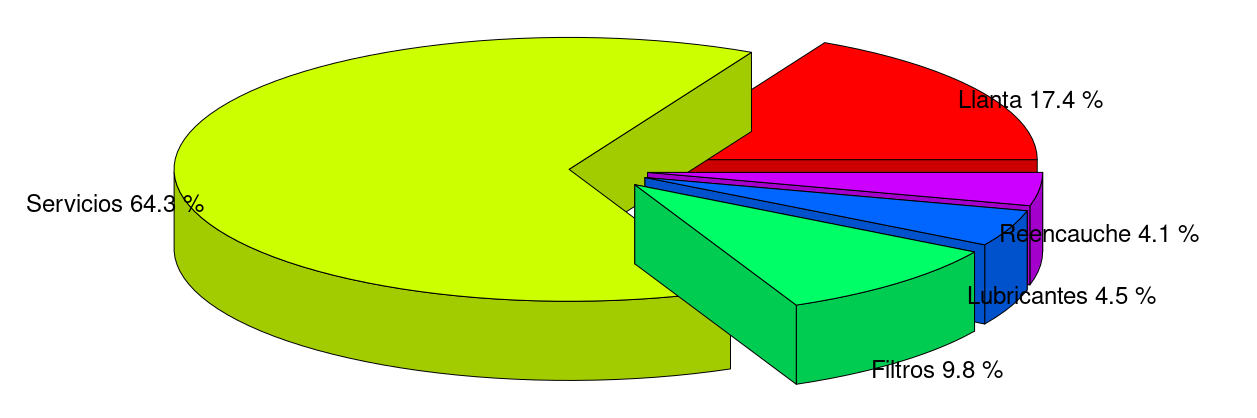
\includegraphics[width=1\textwidth]{img/grafico-pastel-1.png}
                        \caption{Gráfico de barras 5}
                    \end{figure}

            \end{itemize}

    % 4.Conclusiones: ...................................................
    \newpage
    \section{Conclusiones}
        \begin{enumerate}
            \item El uso de R para la limpieza de datos resultó eficaz gracias a la familiaridad con el lenguaje, lo que facilitó la preparación de los datos desde un archivo Excel.
            \item A pesar de la eficiencia en la limpieza, enfrentamos dificultades al representar los datos debido a la falta de experiencia en selección de gráficos y la limitación de tiempo para aprender herramientas gráficas adicionales.
            \item El proyecto destaca la necesidad de fortalecer habilidades en visualización de datos para complementar la limpieza y mejorar la presentación de los análisis.
        \end{enumerate}


    % 5.Bibliografía: ...................................................
    \section{Bibliografía}
        \begin{itemize}
            \item Technologies, R. (2021, 9 diciembre). Cómo crear gráficos básicos con R sin paquetes adicionales. \textit{Geoinnova}. \url{https://geoinnova.org/blog-territorio/crear-graficos-con-r/}
            \item RPubs - Limpieza de datos con R. (s. f.). \url{https://rpubs.com/camilamila/limpieza_R}
        \end{itemize}
    
\end{document}